\section{Case study}
\label{caseStudy}
In this section, we provide a proof-of-concept illustration or scenario composition.
The individual scenarios will use different formalisms to model the ego vehicle, and we will use different tools to verify them.
But first, we give a quick overview of applicable formal verification tools.

Formal verification tools are largely based on two methodologies: model checking, and direct computation of the reachable sets. 
In the former category are UPPAAL, which restricts the model to timed automata, and HyTech, which restricts the model to rectangular hybrid automata. 
Other classes or hybrid systems are decidable, like STORMED systems, but do not currently have tools for their verification.

Several tools exist which explicitly calculate the reachable sets of a dynamical system.
For example, PHAVer and SpaceEx perform reachability analysis on linear hybrid automata. 
The reachability tool Flow* can handle nonlinear hybrid automata, but struggles with large parameter spaces. 
Finally, dReach is an SMT-based solver that answers the question: ``does the system produce a trajectory that enters a given subset $U$ of the state space?''
It is extremely capable, but verification is still time consuming, time bounded, and limited to first order logic. 

We also mention the theorem prover KeYmaeara which has been used for verification of certain driving scenarios.
Because it's a theorem prover, it is an interactive rather than fully automatic tool. 

\subsection{Journey description}
The journey, illustrated in Fig. \ref{fig:scenario} shows the ego vehicle (in gray) driving in the right lane of a uni-directional two lane road network. 
Another car is driving in front of the ego vehicle.
The ego vehicle must eventually initiate a lane change maneuver, which involves moving to the left lane, in order to enter a left hand turn lane.

\begin{figure}[tb]
	\centering
	\label{fig:scenario}
	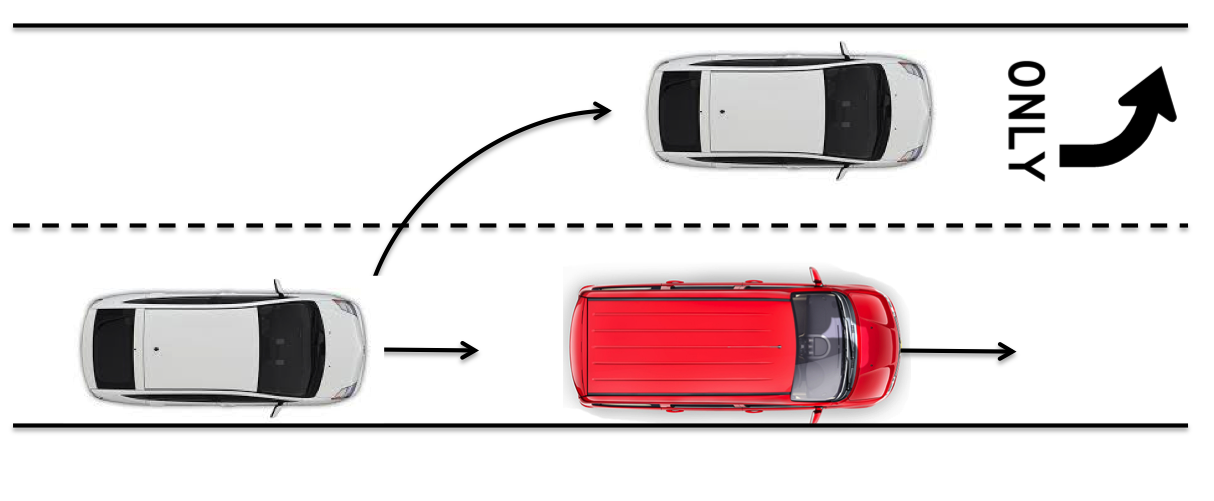
\includegraphics[scale=.4]{scenario.png}
	\caption{Pictorial description of ego vehicle's journey.}
	\label{fig:journey}
\end{figure}

The requirements are:
	\begin{enumerate}
		\item Velocity is always less than or equal to the speed limit
		\item Position is always at a minimum distance from other vehicles in the environment if in the same lane
		\item Eventually, drive a total length of 80m and end up in the left lane.
	\end{enumerate}

\subsection{Scenario 1: lane following}
The first scenario we identify in this journey is the Lane Following scenario. 
First we give the system model.
Both ego and other vehicles are modeled in the same manner. 
First we assume that there is no significant movement of the car along the direction perpendicular to the road's direction, \emph{as long as the vehicle is keeping to its lane}.
Thus the position is given by a scalar $s$.
Therefore, the state of a vehicle is 2-dimensional and given by its position $s$ along the road and velocity $v$: $x = (s,v)$.

A vehicle's dynamics are modeled using a Rectangular Hybrid Automaton: this is a class of hybrid systems where the continuous dynamics in each location are given by so-called rectangular inclusions, namely, $c_1 \leq \dot{x} \leq c_2$ for some rational constants $c_1$ and $c_2$. 
In our case, this means that the vehicles' dynamics are given by 
\[\left[\begin{matrix}
c_{s,1}\\c_{v,1}
\end{matrix}\right]
\leq
\left[\begin{matrix}
\dot{s}\\ \dot{v}
\end{matrix}\right]
\leq
\left[\begin{matrix}
c_{s,2}\\c_{v,2}
\end{matrix}\right]
\]

Thus the velocity $\dot{s}$ and acceleration $\dot{v}$ are bounded.
These are very general dynamics. 
In Section \ref{sec:relating-the-two-system-models} we see how we use this general form to over-approximate the behavior of the accurate nonlinear dynamics of the vehicles.

The elements of the Lane Following scenario are:
\begin{itemize}
	\item $A^1 = \{a\}$ is the set of other agents, in this case consisting of one other agent $a$ (red car in Fig. \ref{fig:journey}).
	\item $Road^1$ is a two-lane unidirectional road segment shown in Fig. \ref{fig:journey}.
	\item $Init^1 = X_{ego}^0 \times X_a$, where 
	$X_{ego} = [0,30] \times [0,1]$ and
	$X_a = [0,36] \times [0,1]$.
	That is, the initial position along the road is anywhere between 0 and 30 meters, and the initial velocity is between 0 and 1 m/s for the ego vehicle. 
	Analogously for the other vehicle.
	\item $\lawSet^1 = \{speedLimit, minSeparation\}$ where
	\[speedLimit \defeq \always (v_{ego} \leq v_{max})\]
	\[minSeparation \defeq \always (s_{ego} \leq s_a - 5)\]
	\item $\goal^1 = \eventually_{[0,30]}(s_{ego} \geq 80)$.
	That is, the ego vehicle must cover 80m in less than 30 seconds.
\end{itemize}

We verified this scenario using HyTech, a model checking tool for rectangular hybrid automata.
The HyTech tool returned the result in .01 seconds on a 32 bit Ubuntu machine on an 1.2 GHz Intel Opteron processor and 600 MB of RAM.

\subsection{Scenario 2: lane change}
The second scenario we identify is a Lane Change scenario.
When the car is performing such dynamic maneuvers with a real chance for safety violation, it is important to work with accurate dynamics, rather than simplified dynamics. 
In this scenario, we model the ego vehicle using a 7D bicycle model of a car, validated on a Cadillac SRX. 
The details of the model are given in the appendix.
We simply note here that the vehicle's position is given by the 2D variable $(s_x,s_y)$, where $s_x$ is the position of the vehicle in the horizontal direction (along the road) and $s_y$ is its position in the vertical direction (perpendicular to the road). 

The other vehicle, on the other hand, is modeled same as in the Lane Following scenario, using a differential inclusion. 
That is because we only care about knowing an envelope around where the other vehicle is.

The scenario elements are given by:
\begin{itemize}
	\item $A^2 = \{a\}$ is the set of other agents, in this case consisting of one other agent $a$ (red car in Fig. \ref{fig:journey}).
	\item $Road^2$ is a two-lane unidirectional road segment shown in Fig. \ref{fig:journey}.
	\item $Init^2 = X_{ego}^0 \times X_a$. 
	Here, $X_{ego}$ is a 7-dimensional subset of $\Re^7$.
	In particular, we consider that state variable $(s_x,s_y)$ starts at (0,0) without loss of generality. And 
	$X_a = [3,10] \times [0,1]$.
	\item $\lawSet^2 = \{speedLimit, minSeparation\}$ where
	\[speedLimit \defeq \always v_{ego} \leq v_{max}\]
	\[minSeparation \defeq \always s_{x,ego} \leq s_{x,a} - 3\]
	\item $\goal^2 = \eventually_{[0,7]}(s_{y,ego} = -W)$.
	That is, the ego vehicle must be in the left lane ($s_y = -W$ in our coordinate system) within 7s.
\end{itemize}

Because the dynamics are now nonlinear, we verify this scenario using dReach, a reachability analysis tool that can handle nonlinear dynamics.
Namely we ask dReach the question: can the system evolve in such a way that the ego vehicle violates its constraints or its goal? 
In this case, dReach returns a negative answer, thus estabilishing the formal correctness of the scenario.

\subsection{Scenario hand-off}
The correctness of the hand-off is established by verifying, using HyTech, that the first scenario either completes successfully (i.e. $\goal^1$ is satisfied), or the system evolves to a point where it satisfies the initialization $Init^2$ of the second scenario.

\subsection{Relating the two system models}
\label{sec:relating-the-two-system-models}
Because we want the two scenarios to be verified for the same underlying ego vehicle, it is important that the dynamics of the ego car in one scenario be an abstraction of its dynamics in the other scenario.
Alternatively, it suffices that they both be abstractions of the same underlying dynamics.
If model $M$ is an abstraction of model $N$, this means that all behaviors of $N$ can be exhibited by $M$. 
Then if $M$ is correct, we know a fortiori that $N$ is correct.

In our case, we over-approximated the nonlinear dynamics of the Lane Change scenario into the Rectangular Hybrid Automaton dynamics of the Lane Following scenario.
Thus we have a formal and verifiable relation between the two models.
